\subsubsection{x86}

\myparagraph{\NonOptimizing MSVC}

Let's compile:

\lstinputlisting{patterns/10_strings/1_strlen/10_1_msvc_EN.asm}

\myindex{x86!\Instructions!MOVSX}
\myindex{x86!\Instructions!TEST}

We get two new instructions here: \MOVSX and \TEST.

\label{MOVSX}

The first one---\MOVSX---takes a byte from an address in memory and stores the value in a 32-bit register. 
\MOVSX stands for \IT{MOV with Sign-Extend}. 
\MOVSX sets the rest of the bits, from the 8th to the 31th, 
to 1 if the source byte is \IT{negative} or to 0 if is \IT{positive}.

And here is why.

By default, the \Tchar type is signed in MSVC and GCC. If we have two values of which one is \Tchar 
and the other is \Tint, (\Tint is signed too), and if the first value contain -2 (coded as \TT{0xFE}) 
and we just copy this byte into the \Tint container, it makes \TT{0x000000FE}, and this 
from the point of signed \Tint view is 254, but not -2. In signed int, -2 is coded as \TT{0xFFFFFFFE}. 
So if we need to transfer \TT{0xFE} from a variable of \Tchar type to \Tint, 
we need to identify its sign and extend it. That is what \MOVSX does.

You can also read about it in \q{\IT{\SignedNumbersSectionName}} section~(\myref{sec:signednumbers}).

It's hard to say if the compiler needs to store a \Tchar variable in \EDX, it could just take a 8-bit register part 
(for example \DL). Apparently, the compiler's \gls{register allocator} works like that.

\myindex{ARM!\Instructions!TEST}

Then we see \TT{TEST EDX, EDX}. 
You can read more about the \TEST instruction in the section about bit fields~(\myref{sec:bitfields}).
Here this instruction just checks if the value in \EDX equals to 0.

\myparagraph{\NonOptimizing GCC}

Let's try GCC 4.4.1:

\lstinputlisting{patterns/10_strings/1_strlen/10_3_gcc.asm}

\label{movzx}
\myindex{x86!\Instructions!MOVZX}

The result is almost the same as in MSVC, but here we see \MOVZX instead of \MOVSX. 
\MOVZX stands for \IT{MOV with Zero-Extend}. 
This instruction copies a 8-bit or 16-bit value into a 32-bit register and sets the rest of the bits to 0. 
In fact, this instruction is convenient only because it enable us to replace this instruction pair:\\
\TT{xor eax, eax / mov al, [...]}.

On the other hand, it is obvious that the compiler could produce this code: 
\TT{mov al, byte ptr [eax] / test al, al}---it is almost the same, however, 
the highest bits of the \EAX register will contain random noise. 
But let's think it is compiler's drawback---it cannot produce more understandable code. 
Strictly speaking, the compiler is not obliged to emit understandable (to humans) code at all.

\myindex{x86!\Instructions!SETcc}

The next new instruction for us is \SETNZ. 
Here, if \AL doesn't contain zero, \TT{test al, al} 
sets the \ZF flag to 0, but \SETNZ, if \TT{ZF==0} (\IT{NZ} stands for \IT{not zero}) sets \AL to 1.
Speaking in natural language, \IT{if \AL is not zero, let's jump to loc\_80483F0}. 
The compiler emits some redundant code, but let's not forget that the optimizations are turned off.

\myparagraph{\Optimizing MSVC}
\label{strlen_MSVC_Ox}

Now let's compile all this in MSVC 2012, with optimizations turned on (\Ox):

\lstinputlisting[caption=\Optimizing MSVC 2012 /Ob0]{patterns/10_strings/1_strlen/10_2_EN.asm}

Now it is all simpler.
Needless to say, the compiler could use registers with such efficiency
only in small functions with a few local variables.

\myindex{x86!\Instructions!INC}
\myindex{x86!\Instructions!DEC}
\INC/\DEC---are \gls{increment}/\gls{decrement} instructions, in other words: add or substract 1 to/from a variable.

\clearpage
\subsubsectionold{\Optimizing MSVC + \olly}
\myindex{\olly}

We can try this (optimized) example in \olly.  Here is the first iteration:

\begin{figure}[H]
\centering
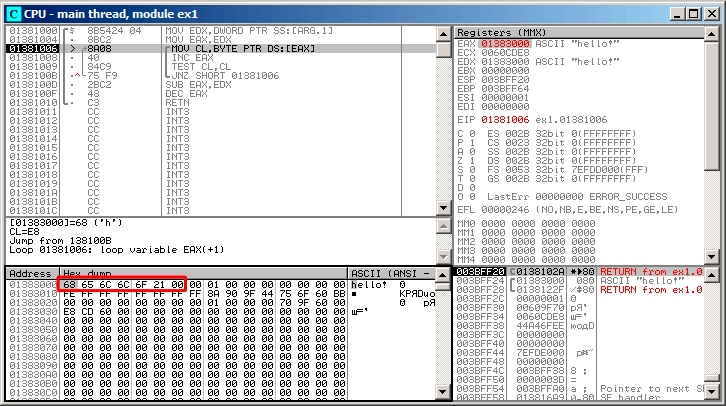
\includegraphics[scale=\FigScale]{patterns/10_strings/1_strlen/olly1.png}
\caption{\olly: first iteration start}
\label{fig:strlen_olly_1}
\end{figure}

We see that \olly found a loop and, for convenience, \IT{wrapped} its instructions in brackets.
By clicking the right button on \EAX, we can choose 
\q{Follow in Dump} and the memory window scrolls to the right place.
Here we can see the string \q{hello!} in memory.
There is at least
one zero byte after it and then random garbage.

If \olly sees a register with a valid address in it, that points to some string, 
it is shown as a string.

\clearpage
Let's press F8 (\stepover) a few times, to get to the start of the body of the loop:

\begin{figure}[H]
\centering
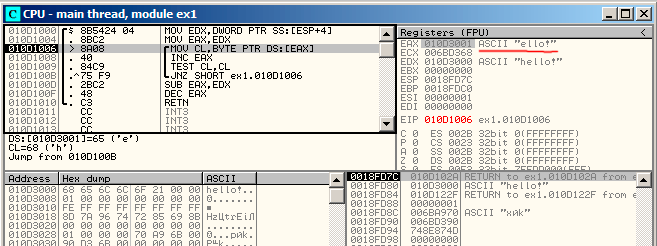
\includegraphics[scale=\FigScale]{patterns/10_strings/1_strlen/olly2.png}
\caption{\olly: second iteration start}
\label{fig:strlen_olly_2}
\end{figure}

We see that \EAX contains the address of the second character in the string.

\clearpage

We have to press F8 enough number of times in order to escape from the loop:

\begin{figure}[H]
\centering
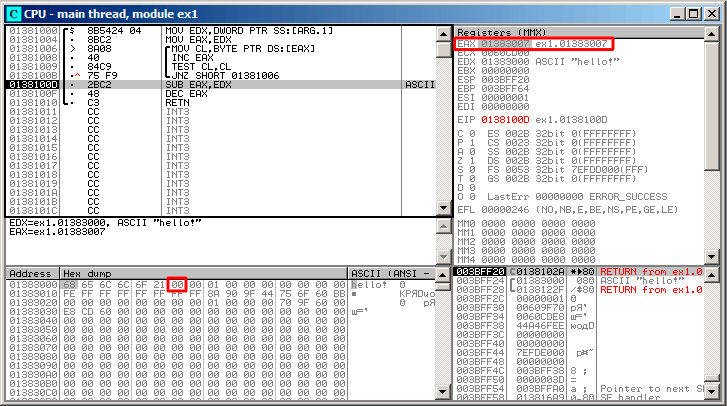
\includegraphics[scale=\FigScale]{patterns/10_strings/1_strlen/olly3.png}
\caption{\olly: pointers difference to be calculated now}
\label{fig:strlen_olly_3}
\end{figure}

We see that \EAX now contains the address of zero byte that's right after the string.
Meanwhile, \EDX hasn't changed,
so it still pointing to the start of the string.

The difference between these two addresses is being calculated now.

\clearpage
The \SUB instruction just got executed:

\begin{figure}[H]
\centering
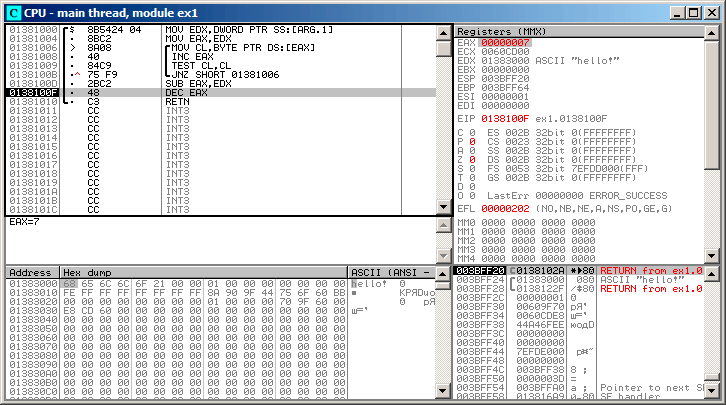
\includegraphics[scale=\FigScale]{patterns/10_strings/1_strlen/olly4.png}
\caption{\olly: \EAX to be decremented now}
\label{fig:strlen_olly_4}
\end{figure}

The difference of pointers is in the \EAX register now---7.
Indeed, the length of the \q{hello!} string is 6, 
but with the zero byte included\EMDASH{}7.
But \TT{strlen()} must return the number of non-zero characters in the string.
So the decrement executes and then the function returns.


\myparagraph{\Optimizing GCC}

Let's check GCC 4.4.1 with optimizations turned on (\Othree key):

\lstinputlisting{patterns/10_strings/1_strlen/10_3_gcc_O3.asm}
 
Here GCC is almost the same as MSVC, except for the presence of \MOVZX.
However, here \MOVZX could be replaced with\\
\TT{mov dl, byte ptr [eax]}.

Probably it is simpler for GCC's code generator to \IT{remember} 
the whole 32-bit \EDX register 
is allocated for a \Tchar variable and it then can be sure that the highest bits has no any noise 
at any point.

\label{strlen_NOT_ADD}
\myindex{x86!\Instructions!NOT}
\myindex{x86!\Instructions!XOR}

After that we also see a new instruction---\NOT. This instruction inverts all bits in the operand. \\
You can say that it is a synonym to the \TT{XOR ECX, 0ffffffffh} instruction. 
\NOT and the following \ADD calculate the pointer difference and subtract 1, just in a different way. 
At the start \ECX, where the pointer to \IT{str} is stored, gets inverted and 1 is subtracted from it.

See also: \q{\SignedNumbersSectionName}~(\myref{sec:signednumbers}).
 
In other words, at the end of the function just after loop body, these operations are executed:

\begin{lstlisting}
ecx=str;
eax=eos;
ecx=(-ecx)-1; 
eax=eax+ecx
return eax
\end{lstlisting}

\dots~and this is effectively equivalent to:

\begin{lstlisting}
ecx=str;
eax=eos;
eax=eax-ecx;
eax=eax-1;
return eax
\end{lstlisting}

Why did GCC decide it would be better? Hard to guess. 
But perhaps the both variants are equivalent in efficiency.
